
\section{Набора изображений, построенных при разном числе итераций и приближении}

\subsection{Множество Мандельброта}
\begin{figure}[h]
    \centering
    \begin{subfigure}{0.30\textwidth}
        \centering
        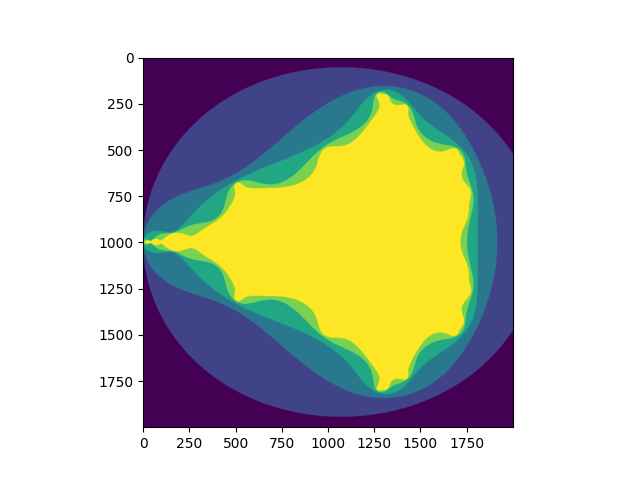
\includegraphics[width=\linewidth]{pic/01.png}
        \caption{Количество итераций - 5}
        \label{fig:mandelbrot_5}
    \end{subfigure}
    \hfill
    \begin{subfigure}{0.30\textwidth}
        \centering
        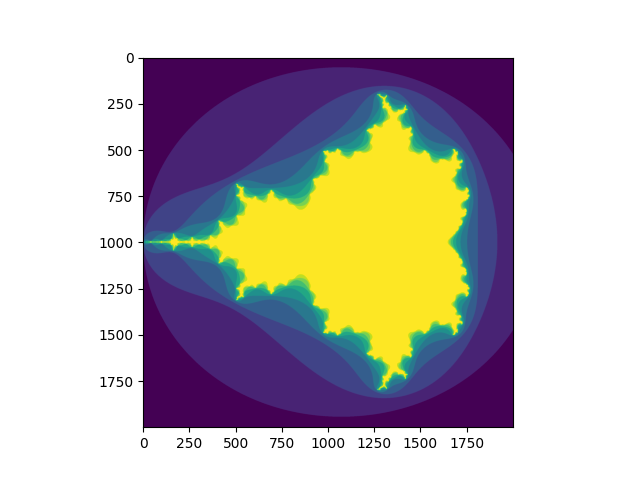
\includegraphics[width=\linewidth]{pic/02.png}
        \caption{Количество итераций - 10}
        \label{fig:mandelbrot_10}
    \end{subfigure}
    \hfill
    \begin{subfigure}{0.30\textwidth}
        \centering
        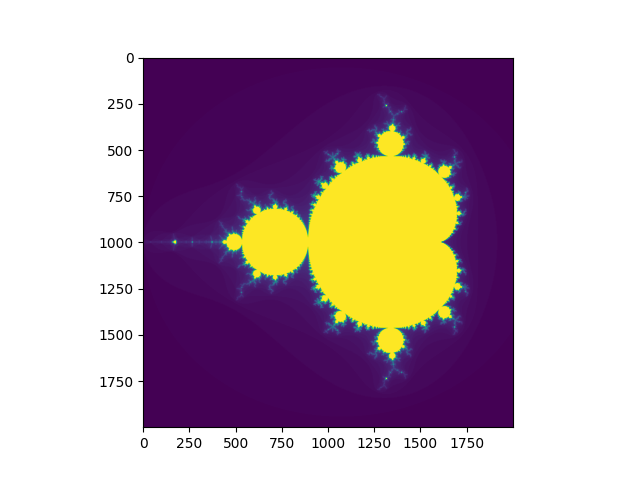
\includegraphics[width=\linewidth]{pic/03.png}
        \caption{Количество итераций - 100}
        \label{fig:mandelbrot_100}
    \end{subfigure}
    \caption{Множество Мандельброта при разном количестве итераций}
    \label{fig:mandelbrot_comparison}
\end{figure}

\begin{figure}[h]
    \centering
    \begin{subfigure}{0.30\textwidth}
        \centering
        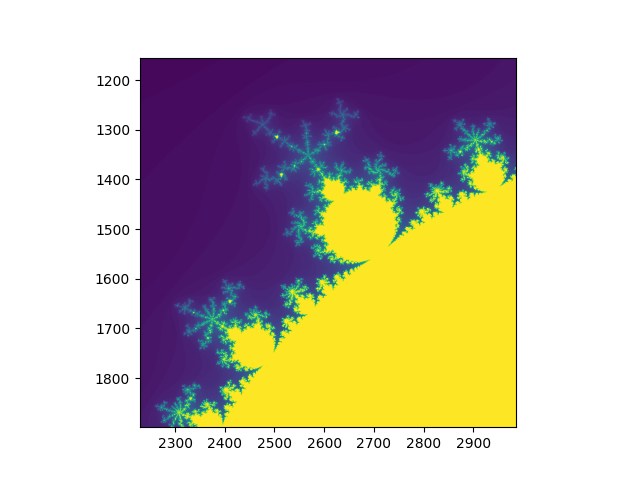
\includegraphics[width=\linewidth]{pic/3.01.png}
        \caption{Деталь 1}
        \label{fig:mandelbrot_detail1}
    \end{subfigure}
    \hfill
    \begin{subfigure}{0.30\textwidth}
        \centering
        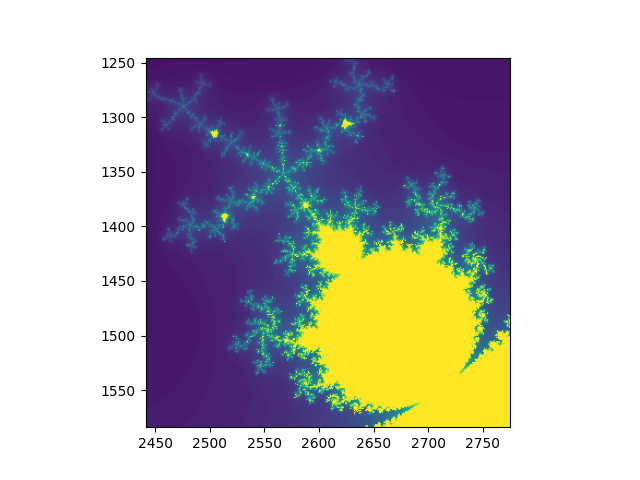
\includegraphics[width=\linewidth]{pic/3.02.png}
        \caption{Деталь 2}
        \label{fig:mandelbrot_detail2}
    \end{subfigure}
    \hfill
    \begin{subfigure}{0.30\textwidth}
        \centering
        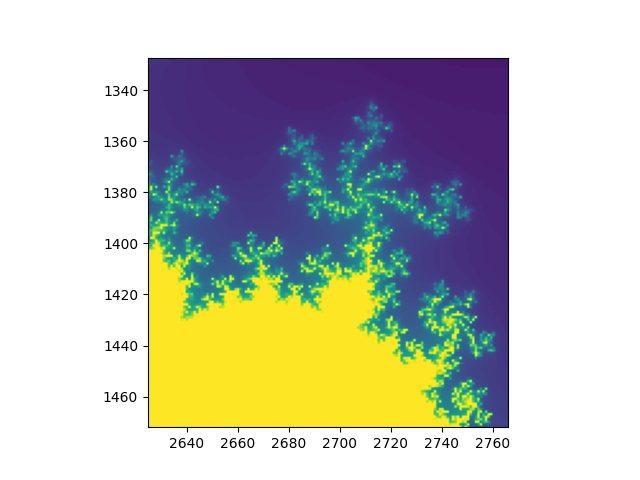
\includegraphics[width=\linewidth]{pic/3.03.png}
        \caption{Деталь 3}
        \label{fig:mandelbrot_detail3}
    \end{subfigure}
    \caption{Фрактальная структура части множества Мандельброта при 100 итерациях}
    \label{fig:mandelbrot_details}
\end{figure}

\subsection{Множество Жюлиа}
\begin{figure}[h]
    \centering
    \begin{subfigure}{0.30\textwidth}
        \centering
        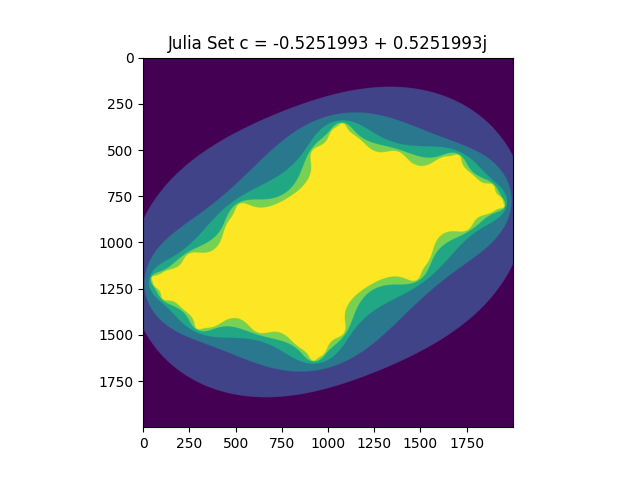
\includegraphics[width=\linewidth]{pic/04.png}
        \caption{Количество итераций - 5}
        \label{fig:julia_5}
    \end{subfigure}
    \hfill
    \begin{subfigure}{0.30\textwidth}
        \centering
        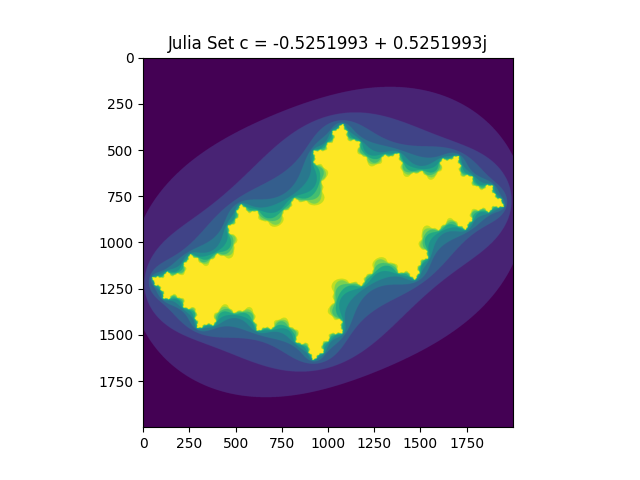
\includegraphics[width=\linewidth]{pic/05.png}
        \caption{Количество итераций - 10}
        \label{fig:julia_10}
    \end{subfigure}
    \hfill
    \begin{subfigure}{0.30\textwidth}
        \centering
        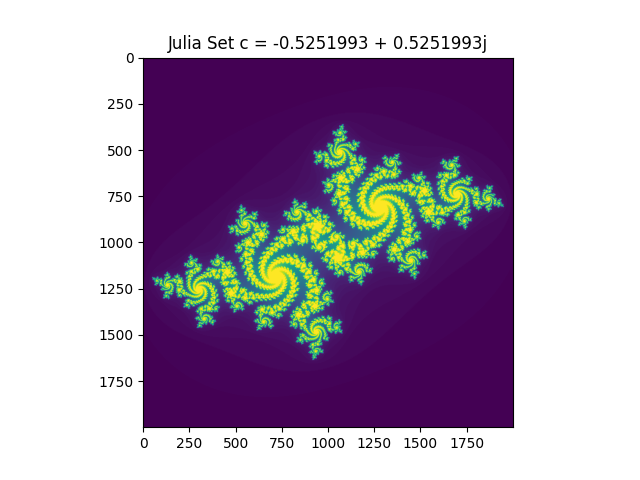
\includegraphics[width=\linewidth]{pic/06.png}
        \caption{Количество итераций - 100}
        \label{fig:julia_100}
    \end{subfigure}
    \caption{Множество Жюлиа(\(c=−0.5251993 +i0.5251993\)) при разном количестве итераций}
    \label{fig:julia_comparison}
\end{figure}

\afterpage{\clearpage}
\begin{figure}[h]
    \centering
    \begin{subfigure}{0.30\textwidth}
        \centering
        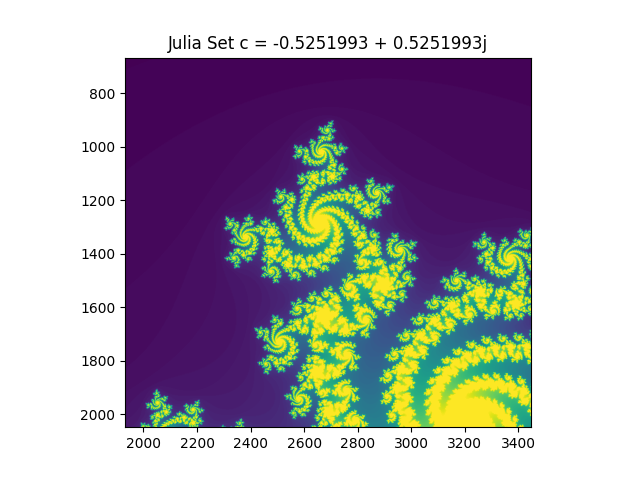
\includegraphics[width=\linewidth]{pic/6.01.png}
        \caption{Деталь 1}
        \label{fig:julia_detail1}
    \end{subfigure}
    \hfill
    \begin{subfigure}{0.30\textwidth}
        \centering
        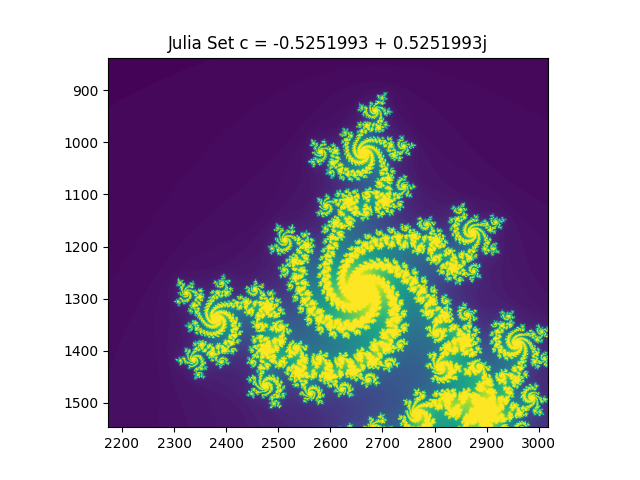
\includegraphics[width=\linewidth]{pic/6.02.png}
        \caption{Деталь 2}
        \label{fig:julia_detail2}
    \end{subfigure}
    \hfill
    \begin{subfigure}{0.30\textwidth}
        \centering
        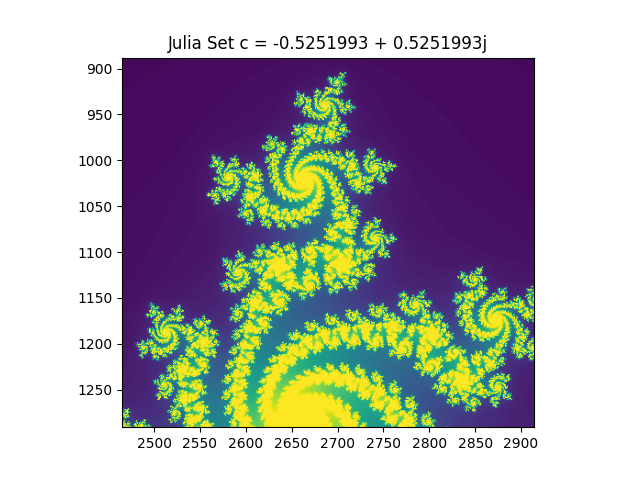
\includegraphics[width=\linewidth]{pic/6.03.png}
        \caption{Деталь 3}
        \label{fig:julia_detail3}
    \end{subfigure}
    \caption{Фрактальная структура части множества Жюлиа при 100 итерациях}
    \label{fig:julia_details}
\end{figure}
